\begin{spacing}{2.0}
    \section{Results and Discussion}

    \subsection{Reaction Coordinates of NaCl Ionic Association in Aqueous Solutions from TICA}
    \label{ssec:tica-results}

    Although $\tilde{\psi}_i$ approximated by TICA will not equal to the actual eigenfunction $\psi_i$ of the transfer operator $\mathcal{T}(\tau)$, 
    the main advantage of TICA is that $\tilde{\psi}_i$ can be computed directly from the correlation of the mean—free collective variables input 
    transformed from any MD trajectory. As each $\tilde{\psi}_i$ is written as a linear combination of the basis function in the collective variable 
    space, $\tilde{\psi}_i$, the contribution from each collective variable to a particular $\tilde{\psi}_i$ can be determined. Figure 
    \ref{fig:tica-timescales} shows the value of the implied relaxation timescale $\tilde{t}_i$, which directly relates to its corresponding 
    $\tilde{\psi}_i$, where the slowest, non—stationary, relaxation timescale ($\tilde{t}_2$) ends at around 60 ps at $\tau = 12$ ps. In this 
    figure, the second slowest relaxation timescale ($\tilde{t}_3$) has the same order of magnitude as $\tilde{t}_2$. Here one could readily see 
    that the first two non—stationary eigenfunctions, $\tilde{\psi}_2$ and $\tilde{\psi}_3$ dominate the dynamics of NaCl in aqueous solution, 
    with a relaxation timescale generally one order of magnitude greater than the next slower eigenfunctions. The shaded area of figure 
    \ref{fig:tica-timescales} represents the area where the implied timescale is less than the lag time; therefore, any eigenfunctions falling 
    within this shaded area are treated as fast processes. Therefore, at $\tau = 4$ ps, there are 6 slowest reaction coordinates according to TICA, 
    2 of which are dominant and 4 others are auxiliary. Similarly, if one consider a long limit of $\tau$ (e.g. at 12 ps), the number of slowest 
    reaction coordinates reduces to 4. Since we are interested in obtaining a better representation of the dynamics, picking the slowest reaction 
    coordinates at $\tau = 4$ ps covers more processes than picking at $\tau = 12$ ps, allowing us to encode the information from these 6 coordinates 
    during the discretization step for building MSM afterwards.

    \begin{figure}[t]
        \centering
        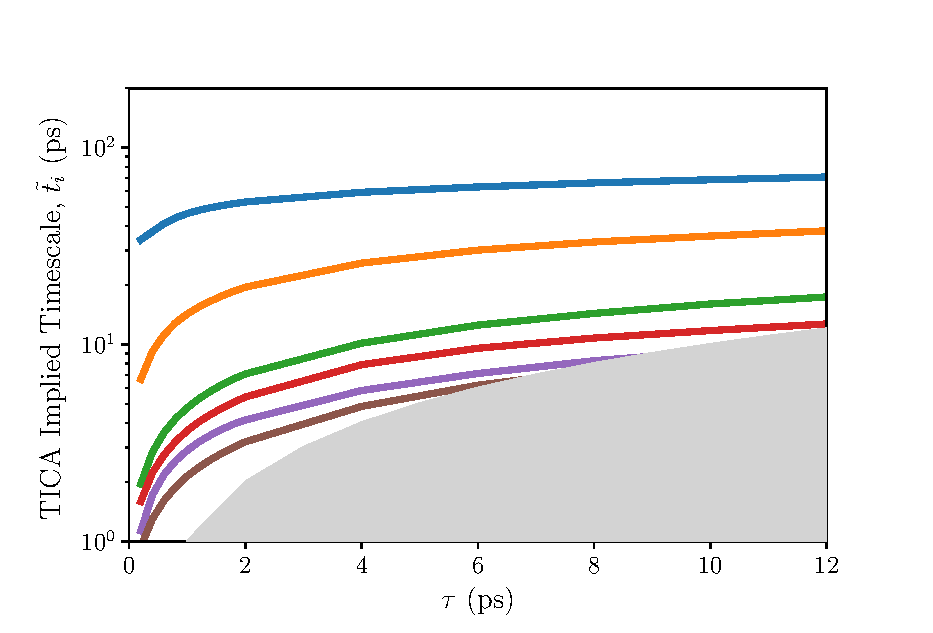
\includegraphics[width=0.85\textwidth]{./figs/fig3-01}
        \caption{Different implied relaxation timescales ($\tilde{t}_i$) corresponding to each specific $\tilde{\psi}_i$ at different values of $\tau$.}
        \label{fig:tica-timescales}
    \end{figure}

    Now that we obtained 6 slowest reaction coordinates from the dynamics with TICA, and we have verified that these 6 reaction coordinates sufficiently
    describe the slowest dynamics by looking at a cumulative kinetic variance of these 6 coordinates. For this set of $\tilde{\psi}_i$, the cumulative
    kinetic variance is found to be 0.997, which is reasonably close to 1. The next question would be how do we describe these coordinates. 
    In particular, we are interested in the first two slowest reaction coordinates as they are very close in relaxation timescales; thus, 
    understanding both of these coordinates would be beneficial for understanding the reaction mechanism for this process. In order to determine 
    the best correlated collective variable with respect to a reaction coordinate, a correlation matrix between the mean—free collective variable 
    inputs and $\tilde{\psi}_i$ can be computed following an equation below,

    \begin{equation}
	C(\xi_i^{MF}, \tilde{\psi}_j) = \frac{1}{\sigma_{\xi_i^{MF}}}\sum_{k=1}^{N_{\xi}} \left[\mathbf{Cov}(\xi_i^{MF}, \xi_k^{MF})\right]^{1/2}\mathbf{U}_{ki}
        \label{eq:features-tic-correlation}
    \end{equation}

    Table \ref{tab:features-tic-correlation} summarizes the correlation between the collective variables to $\tilde{\psi}_2$ and $\tilde{\psi}_3$ 
    computed according to equation \ref{eq:features-tic-correlation}. The result for $\tilde{\psi}_2$ suggests that the 3 features that play important 
    role in this reaction coordinate are $r_{+-}$, $\rho_{ii}$ with $\sigma = r_{+-}$, and $n_B$. The interpretation of this reaction coordinate 
    would have to involve these three collective variables, where the association of the ions would drive the number of water molecules simultaneously 
    associated with the two ions up, changing the water density around the midpoint between the two ions, which is defined from the largest volume 
    possible when the two ions are far apart. However, $\tilde{\psi}_3$, slightly faster in the relaxation timescale than $\tilde{\psi}_2$, mostly 
    involve the changes in water density around the midpoint between the ions significantly more than the association / de-association of the ions. 

    \begin{table}[t]
        \centering
        \caption{Collective variables' correlation with $\tilde{\psi}_2$ and $\tilde{\psi}_3$}\label{tab:features-tic-correlation}
        \begin{tabular}{|c|c|}
            \hline
            \textbf{Feature} & \textbf{Correlation with $\tilde{\psi}_2$} \\ \hline
            $r_{+-}$ & 8.22 \\
            $\rho_{ii}$ ($\sigma = r_{+-}$) & -7.70 \\
            $n_B$ & -6.02 \\
            $\rho_{ii}$ ($\sigma = r_{+-}/4$) & 3.47 \\
            $\rho_{ii}$ ($\sigma = 3.57$ \r{A}) & 3.21 \\
            $\rho_{ii}$ ($\sigma = r_{+-}/2$) & 2.45 \\ \hline
        \end{tabular}
        \quad\quad
        \begin{tabular}{|c|c|}
            \hline
            \textbf{Feature} & \textbf{Correlation with $\tilde{\psi}_3$} \\ \hline
            $\rho_{ii}$ ($\sigma = r_{+-}/3$) & -3.30 \\
            $\rho_{ii}$ ($\sigma = r_{+-}/2$) & -3.19 \\ 
            $\rho_{ii}$ ($\sigma = r_{+-}/4$) & -2.82 \\
            $n_B$ & 1.94 \\
            $r_{+-}$ & 1.71 \\ 
            $n_+^{(1)}$ & -1.65 \\ \hline
        \end{tabular}
    \end{table}

    \begin{figure}[t]
        \centering
        \includegraphics[width=0.8\textwidth]{./figs/fig3-02}
        \caption{Evolution of $\tilde{\psi}_2$ over time as well as $r_{+-}$, $\rho_ii$ ($\sigma = r_{+-}$), and $n_B$}
        \label{fig:time-correlation-psi2}
    \end{figure}

    \begin{figure}[t]
        \centering
        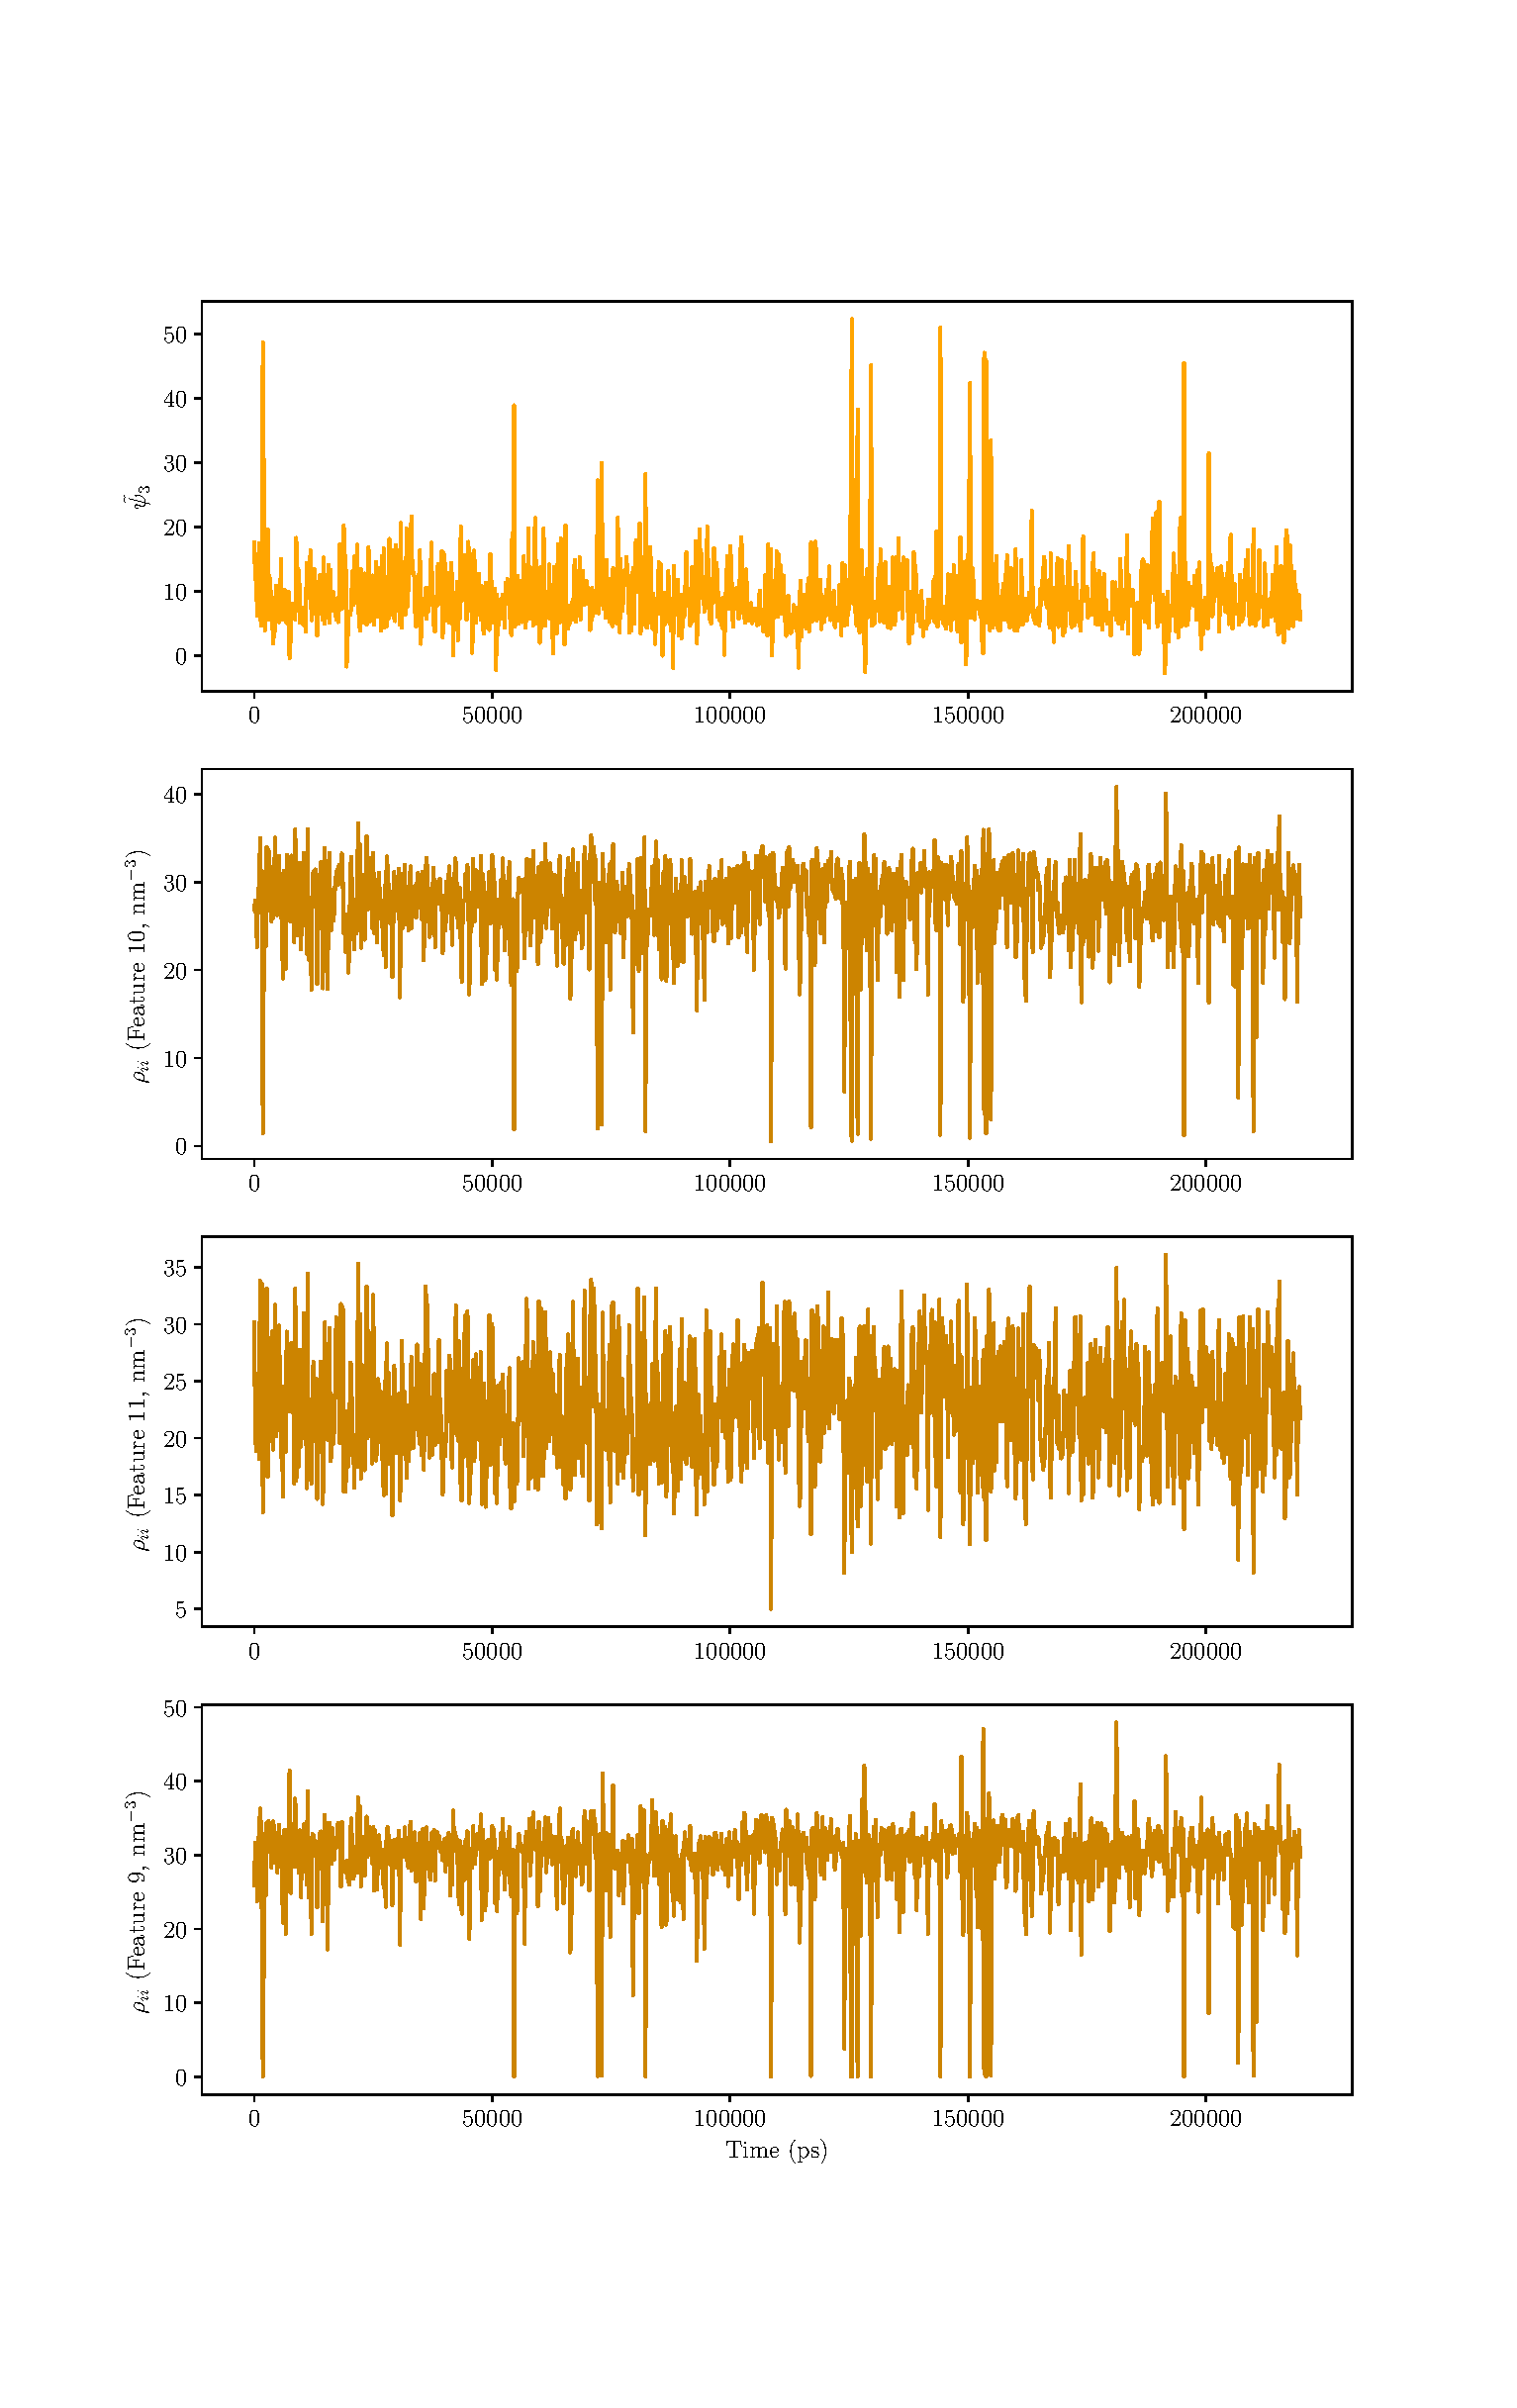
\includegraphics[width=0.8\textwidth]{./figs/fig3-03}
        \caption{Evolution of $\tilde{\psi}_3$ over time as well as $\rho_{ii}$ (Features 10, 11, 9 according to table \ref{tab:features-tic-correlation})}
        \label{fig:time-correlation-psi3}
    \end{figure}

    Figures \ref{fig:time-correlation-psi2} and \ref{fig:time-correlation-psi3} also show a graphical correlation between $\tilde{\psi}_2$ and 
    $\tilde{\psi}_3$ with respect to their 3 dominant collective variables. The time series plots for both $\tilde{\psi}_2$ and $\tilde{\psi}_3$ 
    are consistent with the results we obtained in table \ref{tab:features-tic-correlation}. The slowest motion, $\tilde{\psi}_2$, contains about 
    20 transitions to CIP regions (where $r_{+-}$ is minimum) and several transitions to the SSIP regions (where $r_{+-} \approx 5.0$ \r{A}), and 
    each of these transitions in the inter ionic distance has a pattern in the time series that matches with the evolution of $\tilde{\psi}_2$ over 
    time. Moreover, the evolution of $n_B$ peaks around the same point where $r_{+-}$ is at minimum, while remaining mostly zero throughout the 
    course of the simulation. This result indicates that the CIP configuration of NaCl has to occur in tandem with at least two water molecules 
    simultaneously coordinating with both ions, whereas the region where $n_B = 0$ indicates the bulk region. The SSIP region is usually identified 
    when $r_{+-} \approx 5.0$ \r{A}, where numerous previous literature has consistently found this value from the one—dimensional free energy 
    landscape computation of NaCl in aqueous solutions [CITE], occurs in sync with the region of $n_B \approx 1$, indicating that there is only 1 
    water molecule bridging between the two ions in the SSIP structure.

    According to figure \ref{fig:time-correlation-psi3}, the key transition in this reaction coordinate is observed with collective variables 10, 
    11, and 9 (water density around the midpoint between the ions), all of which correlate strongly with this reaction coordinate. However, the 
    minimum $r_{+-}$ from figure \ref{fig:time-correlation-psi2} does not correlate very well with the high jumps in $\tilde{\psi}_3$, indicating 
    that the association between the ions does not play a key role in this reaction coordinate, which is dominated by the solvent rearrangement 
    around the midpoint of the ions. As this is a slightly faster process than the reaction coordinate $\tilde{\psi}_2$, the rearrangement of the 
    solvent molecules should occur before the association of the ions. It is also interesting to note that in this reaction coordinate, the 
    $n_+^{(1)}$ coordinate also has a slight contribution to this reaction coordinate as well, although not as important as the solvent arrangement 
    between the ions. This finding is consistent with the work of Mullen et al., where they also found that by optimizing a set of three collective 
    variables, the set with maximum likelihood of crossing the two dividing committor surfaces contains either the solvent variables from the water 
    in between or the water density classes, but not from the ion coordination class. The result also indicates that ligand exchange-type reaction 
    is less likely to play an assisted role in the association between the two ions, contrary to the previous hypotheses.

    \placeholder{Matching Pursuit results - put them after comparing eigenvalues between real set and MP set.}
\end{spacing}
